% !TEX root = SoLoud.tex
%===============================================================================

\chapter{Concepts}

\section{Back end}

SoLoud itself "only" performs audio mixing and some resource handling. For it to be useful, it needs one or more sound source and a back end. Some other systems call back-ends 'sink's. Examples of back-ends would be winmm, portaudio, wasapi and SDL audio. SoLoud comes with several back-ends, and is designed to make back-ends relatively easy to implement.

\section{Channel}

One audio stream can contain one or more channels. Typical audio sources are either mono (containing one channel) or stereo (containing two channels), but surround sound audio sources may practically have any number of channels.

\section{Stream}

SoLoud can play audio from several sound sources at once (or, in fact, several times from the same sound source at the same time). Each of these sound instances is a "stream". The number of concurrent streams is limited, as having unlimited streams would cause performance issues, as well as lead to unnecessary clipping.

The default number of concurrent streams - maximum number of "voices" - is 64, but this can be adjusted via a defined constant in the soloud.h file. The hard maximum number is 4096, but if more are required, SoLoud can be modified to support more. But seriously, if you need more than 4096 sounds at once, you're probably going to make some serious changes in any case.

If all channels are already playing and the application requests another sound to play, SoLoud finds the oldest sound and kills it. Since this may be your background music, you can protect channels from being killed by using the soloud.setProtect call.

\section{Clipping}

Audio hardware always has a limited dynamic range. If you think of a signed 16-bit variable, for instance, you can only store values from -32k to +32k in it; if you try to put values outside this range in, things tend to break. Same goes for audio.

\begin{figure}[H]
  \begin{center}
  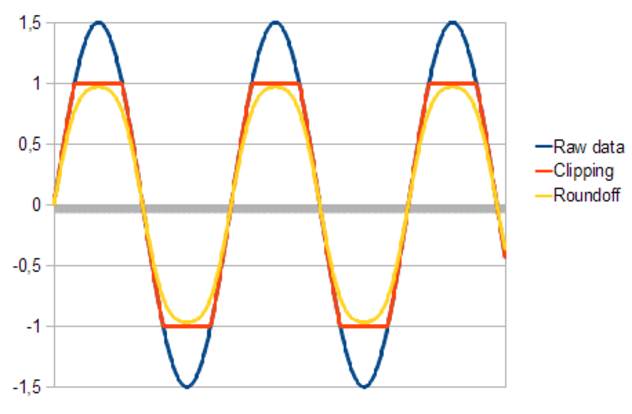
\includegraphics[width=12.0cm]{clipping.pdf}
  \end{center}
\end{figure}
  
SoLoud handles all audio as floats, but performs clipping before passing the samples out, so all values are in the -1..1 range. There's two ways SoLoud can perform the clipping; the most straghtforward is simply to set all values outside this range to the border value, or alternatively a roundoff calculation can be performed, which "compresses" the loud sounds. The more quiet sounds are largely unchanged, while the loud end gets less precision. The roundoff clipper is used by default.

The roundoff clipper does, however, alter the signal and thus "damages" the sound. A more proper way of doing things would be to use the basic clipper and adjust the global volume to avoid clipping. The roundoff clipper, however, is easier to use.

\section{Sample}

The real world has continious signals, whuch would require infinite amount of storage to store (unless you can figure out some kind of complicated mathematical formula that represents the signal). So, we store discrete samples of signals instead. These samples have traditionally been 8, 16 or 24 bit, but high-end audio is tending towards floating point samples.

SoLoud also uses floating point samples internally. First and foremost, it makes everything much simpler, and second, modern computing devices have become fast enough that this is not really an issue anymore.

Floating point samples also take more space than, for instance, 16 bit samples, but memory and storage sizes have also grown enough to make this a feasible approach. Nothing stops the audio sources from keeping data in a more "compressed" format and performing on-the-fly conversion to float, if memory requirements are a concern.

\section{Sample Rate}

The sample rate represents the number of samples used, per second. Typical sample rates are 8000hz, 22050hz, 44100hz and 48000hz. Higher the sample rates mean clearer sound, but also bigger files, more memory and higher processing power requirements.

\section{Play Speed}

In addition to a base sample rate, which represents the "normal" playing speed, SoLoud includes a "relative play speed" option. This simply changes the sample rate. However, if you replace your sounds with something that has a different "base" sample rate, using the relative play speed will retain the effect of playing the sound slower (and lower) or faster (and higher).

\section{Relative Play Speed}

SoLoud lets you change the relative play speed of samples. Please note that asking for a higher relative play speed is more expensive than a lower one.

\section{Resampling}

SoLoud has to perform resampling when mixing. In an ideal case, all of the sources and the destination sample rate are the same, and no resampling is needed, but this is often not true. Currently, SoLoud supports "point sample" resampling, which means it simply skips or repeats samples as needed, as well as "linear interpolation", which calculates linear interpolation of samples. Higher quality resamplers are planned.

\section{Pan}

Where the sound is coming from in the stereo sound, ranging from left speaker only to right speaker only. SoLoud uses an algorithm to calculate the left/right channel volume so that the overall volume is retained across the field. You can also set the left/right volumes directly, if needed.

\section{Handle}

SoLoud uses throwaway handles to control sounds. The handle is an integer, and internally tracks the channel and sound id, as well as an "uniqueness" value.

If you try to use a handle after the sound it represents has stopped, the operation is quietly discarded (or if you're requesting information, some kind of generic value is returned). You can also query the validity of a handle.

\section{Sound Source and Instance}

SoLoud uses two kinds of classes for the sounds. Sound sources contain all the information related to the sound in question, such as wave sample data, while sound instances contain information about an "instance" of the sound.

As an analogue, if you think of an old vinyl record, the sound source is the record, and you can put as many playheads - the instances - on the record. All of the playheads can also move at different speeds, output to a different pan position and volume.

\section{Latency}

Audio latency generally means the time it takes from triggering a sound to the sound actually coming out of the speakers. The smaller the latency, the better.

Unfortunately, there's always some latency. The primary source of latency (that a programmer can have any control over) is the size of audio buffer. Generally speaking, the smaller the buffer, the lower the latency, but at the same time, the smaller the buffer, the more likely the system hits buffer underruns (ie, the play head marches on but there's no data ready to be played) and the sound breaks down horribly.

Assuming there's no other sources of latency (and there quite likely is), with 2048 sample buffer and 44100Hz playback, the latency is around 46 milliseconds, which is tolerable in most cases. A 100ms latency is already easily noticeable.

\section{Filter}

Audio streams can also be modified on the fly for various effects. Typical uses are different environmental effects such as echoes or reverb, or low pass (bassy sound) / high pass (tinny sound) filters, but basically any kind of modification can be done; the primary limitation is the processor power.

SoLoud lets you hook several filters to a single audio stream, as well as to the global audio output.

\section{Mixing Bus}

In addition to mixing audio streams together at the "global" level, SoLoud includes mixing busses which let you mix together groups of audio streams. These serve several purposes.

The most typical use would be to let the user change the volume of different kinds of audio sources - music, sound effects, speech. In this case, you would have one mixing bus for each of these audio source groups, and simply change the volume on the mixing bus, instead of hunting down every sound separately.

When using environmental effects filters, you most likely won't want the background music to get filtered; the easiest way to handle this is to apply the filters to the mixing bus that plays the sound effects. This will also save on processing power, as you don't need to apply the environmental audio filters on every sound effect separately.

It's also possible that you have some very complex audio sources, such as racing cars. In this case it makes sense to place all the audio streams that play from one car into a mixing bus, and then adjust the panning (or, eventually, 3d position) of the mixing bus.